\renewcommand{\password}{key}

\footnote{\se{SUSAN: I am assuming that the intro defines and uses holistic specification and has defined what emergent behaviour is. If it doesn't fit then it needs to start this section.}}
  
In this Section we introduce our problem  through an example and outline our approach.  We work with a  small, object oriented, class-based  language similar to Joe-E \cite{JoeE} with modules,   module-private fields
({accessible} only from   methods {from} the same module),  
and unforgeable and un-enumerable addresses.
Classes have an {implicit} constructor, which   initializes all fields with appropriate default values.
{\prg{Private} methods  {may be} called by objects of the same module,  while \prg{public}  methods  may be called by \emph{any} objects {provided the dynamic types of the arguments are the same as} the formal parameter types.} 
% SD dropped
% Our model of execution is entirely unsurprising with a stack, a heap, and states.
 \footnote{As in Joe-E, we leverage  module-based privacy to restrict propagation of capabilities, and reduce the need for reference monitors etc, \cf Sect 3 in  \cite{JoeE}.}   

% \subsubsection{Internal and external modules, objects, and states}
 \label{s:concepts}

We are concerned with guarantees made in an \emph{open} setting; that is, a given module
$M$ must be programmed so that 
execution of $M$ together with \emph{any} number of external modules $\overline M$
will uphold these guarantees. 
These guarantees must be upheld while 
 $\overline M$, the  \emph{\externalM} modules, are executing; % in contrast, 
 \sdN{they may be} temporarily broken by  the internal module  
tso long as they %are it 
hold {upon entry to external modules.}
 
We therefore distinguish between  \emph{\internalO}
objects --- instances of classes defined in $M$ ---
and \emph{\externalO} objects -- instances of classes defined in any other module.
We also distinguish between
  \emph{\internalC} and   \emph{\externalC} states - those whose receiver is internal or external respectively. 
 
 

\subsection{\prg{Shop} -- illustrating tamed effects} % Reason about external calls (using protection)}
\label{sec:how}

The challenge when calling a method on an external object, is that we have no specification for that method. 
\forget{
However, our  module's %emergent behaviour  
\susan{holistic} specification together with knowledge about the
parameters' lack of access to capabilities %may be used to guarantee that   in order to restrict the possible side-effects of the external call.
can give us the guarantee that  {specific} effects will not take  place, that is they have been tamed.

 \emph{Protection} describes this lack of access to capabilities: An object $o$ is \emph{protected} from $o'$, formally $\protectedFrom {o} {o'}$,  if $o'$ cannot obtain direct access to $o$ unless an internal object affords that access. %to $o$. 
And $o$ is \emph{protected}, formally ${\inside{\prg{\it{o}}}}$, if $o$ is protected from all external objects transitively accessible from the currently executing method call. More in Def. \ref{def:chainmail-protection-from}, and \ref{def:chainmail-protection}.
}
\newcommand{\Mshop}{$M_{{shop}}$\xspace}
 For illustration, consider the following, internal, module \Mshop, and assume that it includes the classes \prg{Item}, \prg{Shop}, \prg{Account}, and \prg{Inventory}. 
Classes  \sdN{\prg{Inventory} and \prg{Item} have the expected functionality. 
\prg{Account}s hold a balance and have a password. 
When given an \prg{Account}'s address, one can pay money into the account, 
and when given an account's address and its password, one can transfer money from that account.
Implementations of these classes appear in the following section.
 \prg{Shop} exports a public method \prg{buy} whose formal parameter \prg{buyer} is an \prg{external}   object.}
 % SD chopped  with a method { \prg{payMe}.}} 

\begin{lstlisting}[mathescape=true, language=Chainmail, frame=lines]
module M$_{shop}$
  ...   
  class Shop
    field accnt:Account, invntry:Inventory, clients: [external]    
  
    public method buy(buyer: external, anItem:Item) -> void
      int price = anItem.price
      int oldBlnce = this.accnt.blnce
      buyer.payMe(this.accnt, price)     // $\red{\mbox{external\ call}}!$
      if (this.accnt.blnce == oldBlnce+price)
         this.send(buyer,anItem)
      else
         buyer.tell("you have not paid me") 
     
      private method send(buyer:external, anItem:Item) -> void  
       ... 
        
\end{lstlisting}
 

The critical point is line 9, where we call the method  \prg{payMe} on \prg{buyer}, passing the shop's account as an argument.
As \prg{buyer} is an external object, we have no method specification for \prg{payMe}. 
\sd{What are the possible effects of that external call?}
% How can we reason about this external call?
\sdN{In particular}, is it possible that the \prg{buyer} will use this opportunity  to drain the shop's account?

\vspace{.3cm}
\noindent
However, if \Mshop provides makes some appropriate guarantees, then  the effects at line 9 are tamed. One can see that
if \Mshop guarantees that \\
$\strut \ \ \ (A)\ \ $ No money can be withdrawn from an account unless the external object causing the\\  
$\strut \ \ \ \ \ \ \ \ \ \ \ $ wirthdrawal can eventually get access to the account's password \\
then \\
$\strut \ \ \ (B)\ \ $ The external  call on line 9 will not cause a reduction in the shop's account's balance.:q


\vspace{.3cm}
The remit of our work is to provide the formal specification and verification tools to support arguments as the one given above. 
\footnote{\sdN{TODO: elaborate here on "can eventually get access", and on "tamed effect"}}
In particular, we need to address the following three challenges:
\begin{description}
\item[1st Challenge] The semantics of "can eventually get access to" 

\item[2nd Challenge] The semantics of "effect will not happen unless .."

\item[3d Challenge] A proof system that allows us to prove that a module satisfies guarantees like those in (A), and that given such guarantees, the effects of the external call are tamed.
\end{description}


\forget{
 If our internal module has a holistic specification (which uses \{ \} brackets around propositional assertions) that says that the balance of the \prg{Account} does not decrease unless there is unprotected access to its key, that is:
 
% $\strut\ \ \ \ \ S_0\ \  \triangleq \ \ \TwoStatesN{ \prg{a}:\prg{Account},\prg{b}:\prg{int} } {\inside{\prg{a.key}} \wedge \prg{a.\balance} \geq \prg{b} } $

$$\TwoStatesN{ \prg{a}:\prg{Account},\prg{b}:\prg{int} } {\inside{\prg{a.key}} \wedge \prg{a.\balance} \geq \prg{b} } $$

\noindent 
%where \inside{\prg{a.key}}  means that account \prg{a}'s key is protected from external calls, 
we claim that the call \emph{is} safe!  At line 6 the \password~was protected from the \prg{buyer}, so after the external call -- \ie after line 9 --  the  balance of the shop's account will not have decreased.
 
 \forget{  
 \susan{ Up to now we only know about module-wide specifications. I think you need to introduce where the Hoare triple comes from in your specification language. 
\sdN{The below is not a spec, it is only a  "classic" Hoare triple, the only novelty is that it uses $ \protectedFrom {\prg{this.\myAccount.key}}$ in the assertion.  I  think that the reader will expect something like Hoare logic. Let us see how the introduction works, and then we decide.}
 Also the triangle operator needs more justification of why you need to change the viewpoint to verify the specification. \sdN{
 Wrt to justification of triangle, I expanded the para starting with "While ..." . Can we make it more explicit?}}
 }
  
 {Proving this introduces new challenges: We want to  establish something like the Hoare triple\\
$\strut \ \ \ \ \ \ \ \ \ \ \  \{\  \ {\protectedFrom {\prg{this.\myAccount.key}} {\prg{buyer}}\ \wedge\ {\prg{this.\myAccount.\balance}}=\prg{b}    }\ \  \}$\\
$\strut \ \ \ \ \ \ \ \ \ \ \   \ \ \ \ \ \ \ \ \ \ \ \ {\ \prg{buyer.payMe(this.accnt,price)}   \ } $\\
$\strut \ \ \ \ \ \ \ \ \ \ \  \{\  \ \  {\prg{this.\myAccount.\balance}} \geq  \prg{b} \  \  \}$ 
}
\\
 {%We want to use $S_4$. 
To apply our specification, we need to establish  ${\inside {\prg{this.\myAccount.key}}}$, and  $\prg{this.\myAccount.\balance}\geq\prg{b}$. 
The latter can be done through the rule of consequence. 
But what about the former? 
We only know that $\protectedFrom {\prg{this.\myAccount.key}} {\prg{buyer}}$, but   need the stronger property  ${\inside {\prg{this.\myAccount.key}}}$.}

 {While we cannot be certain that \prg{this.\myAccount.key} is  protected during the execution of \prg{buy}\footnote{What if one of the \prg{clients} had access to it?}}, we are certain that it  \emph{is} protected during the execution of \prg{payMe}: 
This is so, because the   accessible objects in the execution of \prg{payMe} are those accessible from \prg{buyer}.
In general, more objects are protected from the viewpoint of the callee than from the viewpoint of the caller. 
To express this, we define the operator $\pushSymbolAA$ , which   translates an assertion from the viewpoint of the callee, to that of the caller:
 $\PushAS y A$   guarantees that $A$ will hold when the values of variables $\overline y$ have been pushed onto a new frame. 
 In particular,   $\PushAS y {(\inside \re)} =  \protectedFrom \re {\overline {y} }$ for any term  $\re$ -- \cf 
 Def. \ref{def:push},  and Lemma \ref{lemma:push:ass:state}.
Here we have that 
 $\PushASLong {\{\prg{buyer},\prg{price}\}}  {(\inside {\prg{this.\myAccount.key}})}$
 =  $\protectedFrom {\prg{this.\myAccount.key}} {(\prg{buyer},\prg{price})}$.

\forget{
 {Below we show a simplified version of a Hoare logic rule %\ruleExtCallB\ from
dealing with external calls -- \cf. Fig.\ref{f:external:calls} }
 
 $\inferruleNoName  
 	{ 
   	   {\TwoStatesN {\overline {x:D}} {A}}\ \   \mbox{is part of $M$'s specification}
        }
	{   \triple { \    { \external{y_0}} \,     \wedge \,  \overline{x:D}\  \wedge\  {\PushAS {y}{A}}\ }  
						{ \ u:=y_0.m(y_1,.. y_n)\    }
						{ \    {\PushAS {y}{A}}  \ }
						\  \  ...
         }
$
}

\forget{
\vspace{.1cm}
  \noindent
 \textbf{NOTES}
 \notesep Requiring that the account's key was protected from all external objects would be far too strong; if that were the case, then the account would not be useful for any payments.
 \notesep Requiring that the account's  key was protected at the time of the call of \prg{buy} would also be far too strong: our module cannot impose restrictions on the callers' external state  upon the call to \prg{buy}.
 \notesep 
 We could specify the method \prg{buy} through the pre-condition $\protectedFrom {\prg{a.key}} {\prg{buyer}} \wedge {\prg{a.\myAccount.\balance}}=\prg{b}$ which
 guarantees that $\prg{a.\myAccount.\balance}\geq \prg{b}$.  Note that this is a  direct conclusion of $S_4$; 
  as \prg{Shop} is part of our internal module, this specification is superfluous -- more in Ex. \ref{example:mprepost}.\footnote{TODO need to re-introduce spec inference in the main text}
 }
}
 
\subsection{1st Challenge: eventual access} 

We introduce the concept of protection to  describes a lack of access to capabilities: 
 \begin{description}
\item[Protection] An object $o$ is \emph{protected} from $o'$, formally $\protectedFrom {o} {o'}$,  if $o'$ cannot obtain direct access to $o$ unless an internal object affords that access. %to $o$. 
Object $o$ is \emph{protected}, formally ${\inside{\prg{\it{o}}}}$, if $o$ is protected from all external objects transitively accessible from the currently executing method call. More in Def. \ref{def:chainmail-protection-from}, and \ref{def:chainmail-protection}.
 \end{description}
 
Figure \ref{fig:ProtectedBoth} illustrates  these concepts.  In the left pane,   $o_1$, $o_4$, $o_5$ and $o_9$ 
are protected from $o_2$.
 The middle pane's  top frame is  $\phi_1$; it has one  variables,   \prg{this},  pointing to $o_1$; here 
 $o_1$, $o_2$, $o_4$, $o_5$ and $o_9$  are protected. 
 The right pane's  top frame is  $\phi_2$; it has two  variables,   \prg{this},  and \prg{x}, pointing to $o_3$ and  $o_7$ resp;
  in addition  to  the objects protected in the previous pane, objects $o_3$ and $o_7$ are protected.


\begin{figure}[htb]
\begin{tabular}{|c|c|c|}
\hline
\resizebox{4.5cm}{!}{
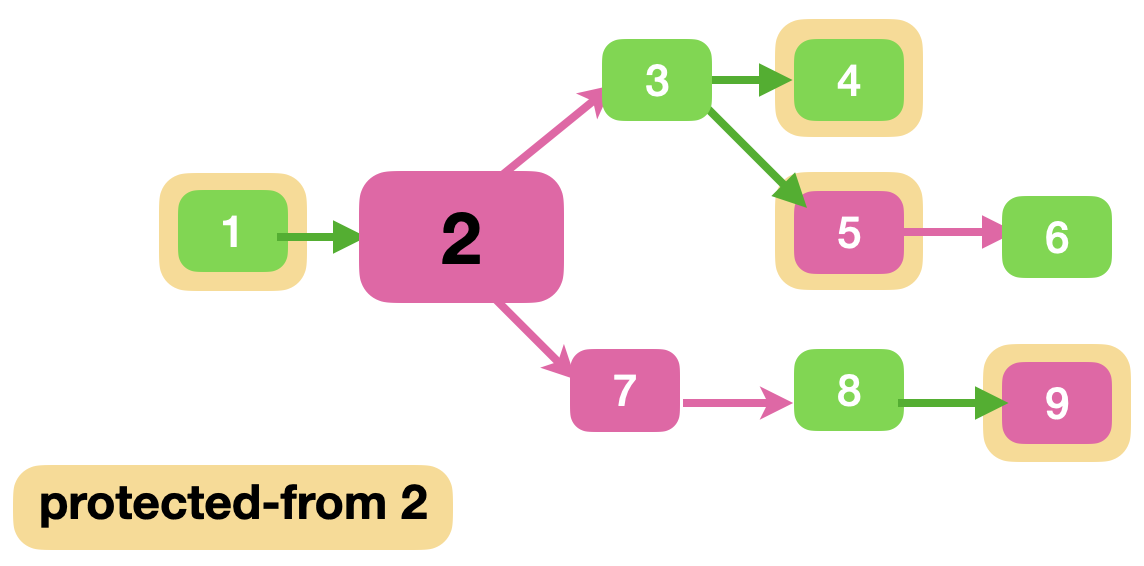
\includegraphics[width=\linewidth]{diagrams/prfC.png}
} 
&
\resizebox{4.5cm}{!}{
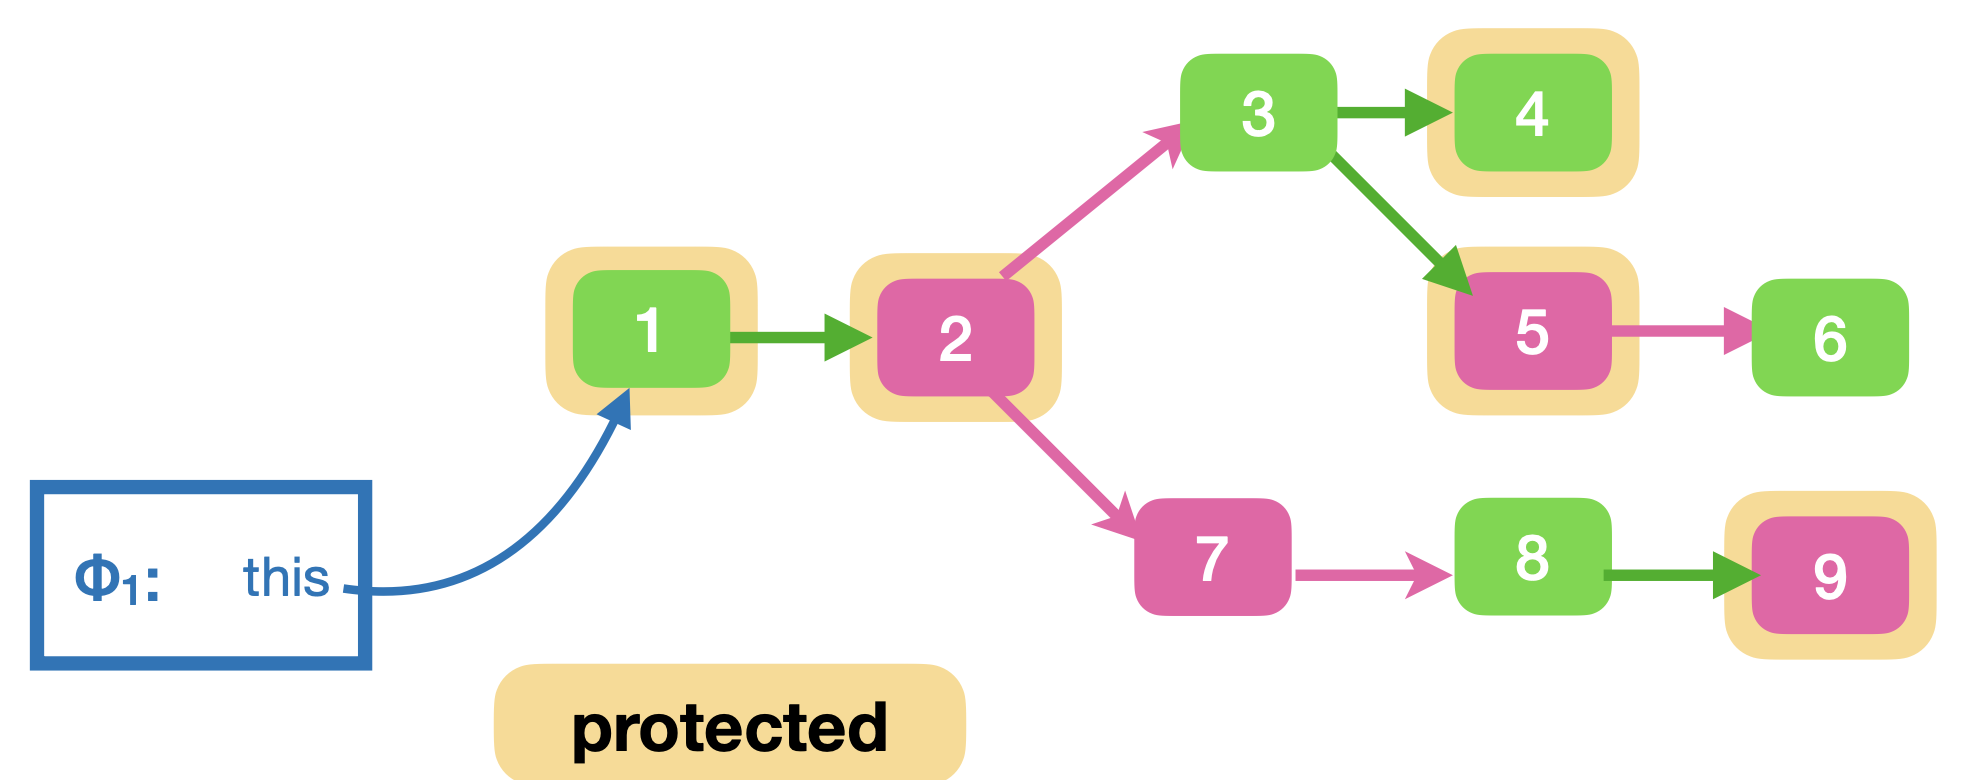
\includegraphics[width=\linewidth]{diagrams/prtFirst.png}
}
&
\resizebox{4.5cm}{!}{
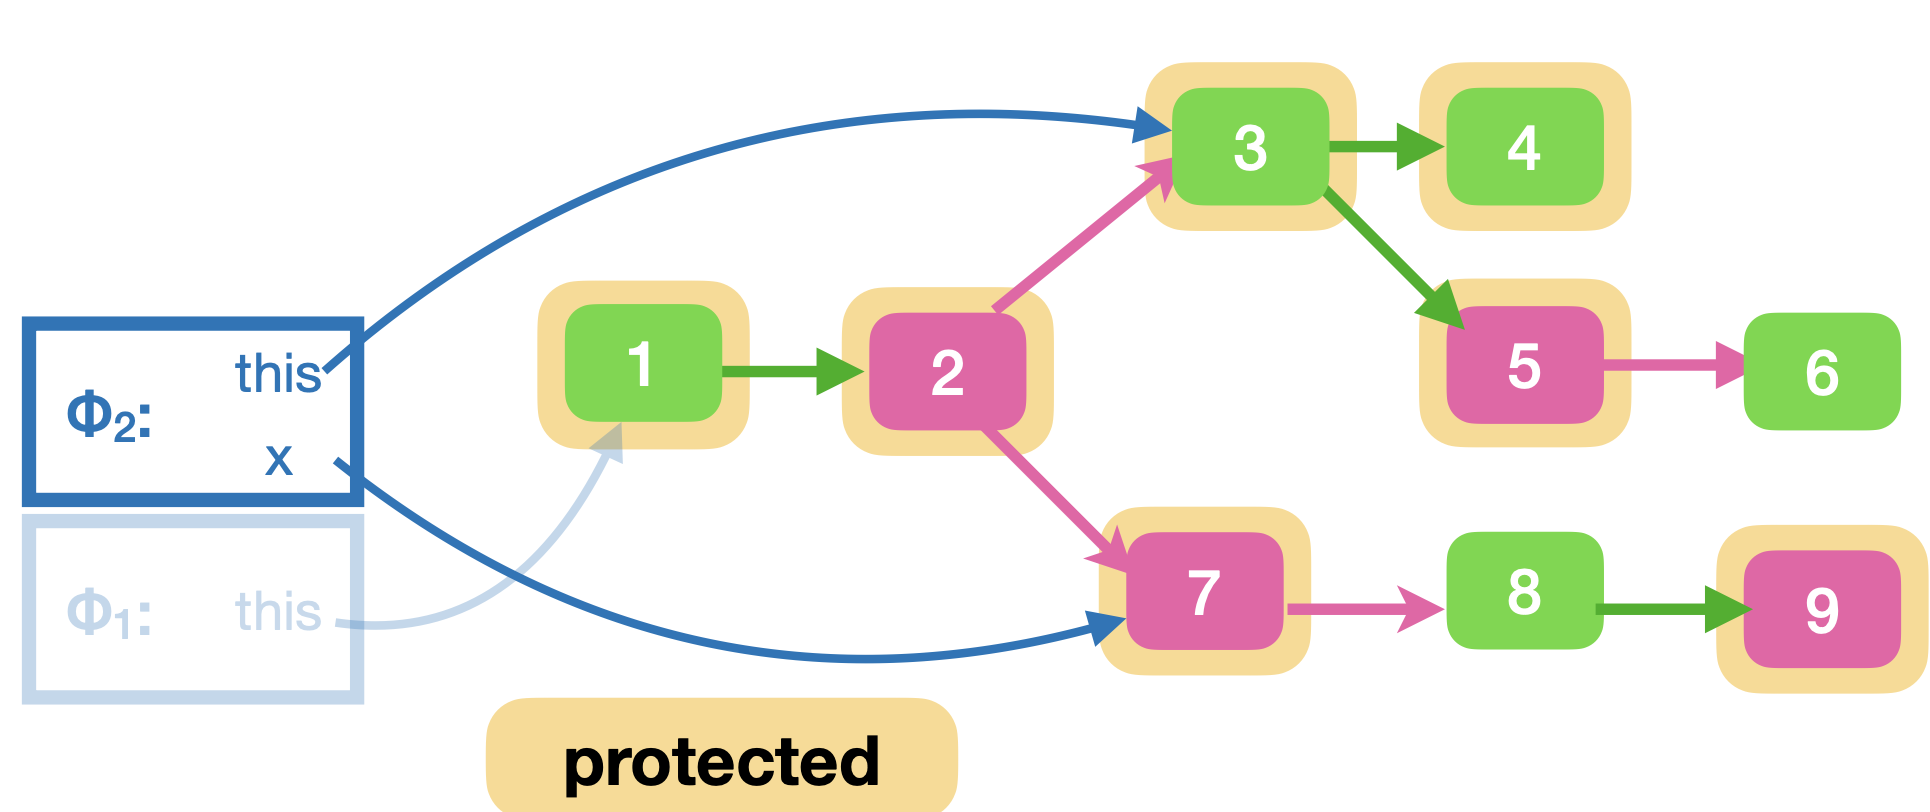
\includegraphics[width=\linewidth]{diagrams/prtSecond.png}
}
\\
\hline
protected from object $o_2$
&
protected  with top frame $\phi_1$
&
protected  with top frame $\phi_2$
\\
\hline \hline
\end{tabular}
   \caption{Protected from, and Protected. Pink resp. green squares are external resp. internal objects. Connecting straight arrows  indicate fields. Blue boxes are frames on the stack. Protected objects   highlighted in yellow.}
   \label{fig:ProtectedBoth}
 \end{figure}
 

\subsection{2nd Challenge: Specification of tamed effects}

How to express the guarantee that some effects will not happen? In particular, when such effects can be the outcome of the execution of more than one method? Traditional PRE/POST condition specifications cannot express guarantees that two or more of our methods won't interact to produce an untamed effect. 

Instead, we build on the concept of two-state invariants, and define

\begin{description}

\item[{Scoped invariants}] describe emergent behaviour:  {$\TwoStatesN  {\overline{x:C}}  {A}$} expresses that if a 
% SD: drop reachable, as we not define it here, and it is not that fundamental, I think
{state} $\sigma$ 
  satisfies ${\overline{x:C}}  \wedge A$, then all $\sigma$'s \emph{scoped} future  states will  {also} satisfy  {$A$}. 
The scoped future  {contains all states which can be reached through any steps, including further method calls and returns, but stopping before returning} from the call active in $\sigma$ --  \cf. Def  \ref{def:shallow:term}.
% SD removed the below because it seems to talk both about the meaning of  {$\TwoStatesN  {\overline{x:C}}  {A}$}  and scoped future.
% I was confused when I read it
% in other words, the current call \emph{scopes} where \se{$A$} must hold -- more in Def 3.1. 
\sdM{We} consider executions of the internal module linked with any number of unknown, external modules,
-- \cf Sect. \ref{sect:execution}.
 For $\sigma$ and its scoped future   we only consider external states -- \cf Def \ref{def:necessity-semantics}.

\end{description}

    
%    \subsection{Challenge: Specify code that tames emergent behaviour} % of modules}
\label{s:bank}

\noindent
For example, the following scoped invariants\\
\label{s:bankSpecEx}
%{
% \begin{tabular}{lcll}
%
$\strut\ \ \ \ \ S_1\ \  \triangleq \ \ \TwoStatesN {\prg{a}:\prg{Account}}  {\inside{\prg{a}}} $ 
\\
$\strut\ \ \ \ \  S_2\ \  \triangleq \ \ \TwoStatesN  {\prg{a}:\prg{Account}}  {\inside{\prg{a.pwd}}} $ 
 \\
$\strut\ \ \ \ \  S_3\ \  \triangleq \ \ \TwoStatesN {\prg{a}:\prg{Account},\prg{b}:\prg{int}}  {\inside{\prg{a}} \wedge \prg{a.\balance}=\prg{b}}  $
\\
$\strut\ \ \ \ \  S_4\ \  \triangleq \ \ \TwoStatesN{ \prg{a}:\prg{Account},\prg{b}:\prg{int} } {\inside{\prg{a.pwd}} \wedge \prg{a.\balance} \geq \prg{b} } $
 
% \end{tabular}
%}

\noindent
%specifications
 give the  guarantees:\\
 $\strut\ \ \ \ \ S_1$:\   accounts are not leaked, \\
$\strut\ \ \ \ \ S_2$:\    keys are not leaked,\\
$\strut\ \ \ \ \ S_3$:\  the balance is not modified unless there is unprotected access to the account,  \\%while 
$\strut\ \ \ \ \ S_4$:\   the balance does not decrease unless there is unprotected access to the key.  


%Having protection to limit access from external modules is necessary to tame the use of our code by potentially hostile external modules. We also need to make sure that our code doesn't accidentally leak effects.  Traditional PRE/POST condition specifications cannot express guarantees that two or more of our methods won't interact to produce an untamed effect. We use an example from \cite{XXXELang,FASE} to demonstrate this  \emph{emergent behaviour} and show how our holistic specifications, similar to those proposed in \cite{OOPSLA22}, which must hold whenever an external module is executing our code, can be used to tame effects.

\vspace{.2cm}

\begin{example}
To illustrate the meaning of these specifications, we show three versions of a bank account class that is part of our internal module \Mshop. To differentiate between the three we rename \Mshop  as $\ModA$,  $\ModB$, or $\ModC$.
All versions {use the same method to} allow the withdrawal of money, only when supplied with the key to the account.
Moreover, in $\ModA$ the key is immutable, in $\ModB$ it is unconditionally mutable, while in $\ModC$ the key may be modified, but only if supplied with the old key. 



%\emph{Guarding} is the crucial expectation that comes with object capabilities. \footnoteSD{SAY THIS BETTER?} 
%Hoare logics support the specification of    enabling of effects (through per-method PRE/POST-condition pairs), but not of guarding of effects.
%The latter % specification of capabilities as guards 
%requires per-module guarantees, as proposed, \eg,  in \cite{OOPSLA22}, and in also the current work.
%\footnoteSD{BOLD! Birkedahl and Dreyer might scream!}
%
% \vspace{.1cm}
\begin{lstlisting}[mathescape=true, language=Chainmail, frame=lines]
module $\ModA$      
  class Shop   ... as earlier ...
  
  class Key
  
  class Account
    field blnce:int 
    field key: Key
    public method transfer(dest: Account, key': Key, amt: int) -> void
      if this.key==key'
        this.blnce-=amt
        dest.blnce+=amt
     public method set(key': Key) -> void
      if this.key==null
        this.key=key'
\end{lstlisting}

Now consider  module \ModB, which allows any client to reset an account's key at any time.  \ModC, on the other hand  requires the existing key in order to change it.
  
  

\begin{tabular}{lll}
\begin{minipage}[b]{0.42\textwidth}
\begin{lstlisting}[mathescape=true, language=Chainmail, frame=lines]
module $\ModB$
   ... as earlier ...
 
   class Account
    field blnce:int 
    field key: Key 
    public method transfer(..) ...
      ... as earlier ...
    public method set(key': Key)
      this.key=key'
      $\ \ \ $
\end{lstlisting}
\end{minipage}
&\ \ \  \ \   &%
\begin{minipage}[b]{0.45\textwidth}
\begin{lstlisting}[mathescape=true, language=chainmail, frame=lines]
module $\ModC$
  ... as earlier ...

  class Account
    field blnce:int 
    field key: Key
    public method transfer(..) 
      ... as earlier ...
    public method set(key',key'': Key)
      if (this.key==key') 
        this.key=key''
\end{lstlisting}
\end{minipage} 
\end{tabular}

{Thus, in all three modules, the key is an object capability which \emph{enables} the withdrawal of the money. 
Moreover, in $\ModA$ and $\ModC$, the key
\sdN{is a capability} used to  \emph{tame} withdrawal of money, preventing those without it from getting the money from the account.}

Crucially however,  in $\ModB$ the key \emph{does not tame} withdrawal of money.
Using $\ModB$, it is possible to start in a state where the account's key is unknown, modify the key, and then withdraw the money. 
% This is not possible  in $\ModA$ and $\ModC$.
% \noindent
Although the \prg{transfer} method is the same in
all three modules,   code  {such as}
\\ 
$\ \strut \hspace{.2in} $ \prg{k=new Key;  acc.set(k); acc.transfer(rogue\_accnt,k,1000)} 
\\ 
is enough to drain  \prg{acc} in \ModB without knowing the \password.\footnoteSD{CAREFUL: we had 
$\ \strut \hspace{.01in} $ \prg{an\_account.set(42); an\_account.transfer(rogue\_accnt,42)} but this was type incorrect!}
%
%This example demonstrates that we need to consider the 
\emph{Emergent behaviour} is key here: 
Even though the method \prg{transfer} in  \ModB is ``safe'' when considered in isolation, it is not safe when considered in conjunction with other methods from the same module. 

\vspace{.2cm}
Fortunately, our holistic  specifications  rule  out \ModB while permitting \ModA and
\ModC. Namely
all three modules satisfy $S_1$ and $S_3$. However, $\ModA$ and $\ModC$ also satisfy $S_2$ and $S_4$, while $\ModB$ satisfies neither $S_2$ nor $S_4$.
\end{example}
 \vspace{1cm}
 \sdN{SD: I have stopped the restructuring here}
 
  \subsection{3rd Challenge:  Proving that a module adheres to its specification} %  (using scoped invariants)}
 \label{sec:howThird}
 
 The holistic specifications we have shown are all of the form {$\TwoStatesN  {\overline{x:C}}  {A}$.
These are  \emph{scoped invariants} and are used when describing emergent behaviour:  {$\TwoStatesN  {\overline{x:C}}  {A}$} expresses that if a state $\sigma$ 
  satisfies ${\overline{x:C}}  \wedge A$, then all $\sigma$'s \emph{scoped} future  states will  {also} satisfy  {$A$}. 
The scoped future contains the states which can be reached through all steps, including further method calls and returns, but stopping before returning from the call active in $\sigma$ --  \cf. Def  \ref{def:shallow:term}.
We consider executions of the internal module linked with any number of unknown, external modules,
-- \cf Sect. \ref{sect:execution}.
 For $\sigma$ and its scoped future   we are only interested in external states -- \cf Def \ref{def:necessity-semantics}.
\forget{If $\sigma$ is executing a call to a public method of our module, then the external state $\sigma'$ may be reachable after the termination of that method, but also through further external calls made within that method.}
 
\Eg if $\sigma$ was an external state executing a call to \prg{Shop::buy}, then $\sigma'$ could be an external state reachable 
after the return from \prg{Shop::buy}, but could also be reachable
during execution of the external call \prg{payMe}.
This means that we are  interested in the states before and after a method (or statements), but  also  in the external states reachable during execution of that method (or statements).
To accommodate this, we extend   traditional Hoare triples to quadruples of the form\\
 $\strut \ \hspace{4cm} \quadruple {A} {\, stmt\, }{A'} {A''}$\\  
 % These promise 
 promising that terminating execution of $stmt$ in  states satisfying $A$  reaches  a  final state satisfying $A'$, and any intermediate external states reachable during execution of $stmt$ satisfy    $A''$ -- \cf Def. \ref{def:hoare:sem}.

\vspace{.1cm}

We assume a  Hoare logic of  triples, and define an embedding into our quadruples. 
We then extend it with substructural rules, rules talking about protection, internal and external calls, 
and the module's adherence to its 
specification - more in Figs. \ref{f:underly} -  \ref{f:calls}. % \ref{f:wf}.
Our Hoare logic rule dealing with external calls is:
 
 $\inferruleNoName  
 	{ 
   	   {\TwoStatesN {\overline {x:D}} {A}}\ \   \mbox{is part of $M$'s specification}
        }
	{   \quadruple { \    { \external{y_0}} \,     \wedge \,  \overline{x:D}\  \wedge\  {\PushAS {y}{A}}\ }  
						{ \ u:=y_0.m(y_1,.. y_n)\    }
						{ \    {\PushAS {y}{A}}  \ }
						{\  A  \ }
         }
$
 
 \vspace{.2cm}
A module is well-formed, if  its invariants are well-formed,  all  its public methods preserve each of its invariants, and  all its methods satisfy their specifications - \cf  Fig.  \ref{f:wf}.
%
An invariant is well-formed if % the constituent assertion 
it is \emph{encapsulated}, \ie can only be invalidated by code from that module -- \cf Def. \ref{d:encaps}. 
%For example, in \ModA the assertion  \prg{a.balance}$\geq$\prg{b} is encapsulated, but it would not be encapsulated 
%% in a module \ModD   implements balances through a third party, openly accessible ledger 
%if balances were in an external, openly modifiable ledger -- \cf Ex. \ref{ex:not:encaps}.
% 
A method preserves an assertion   if it preserves it across its pre- and post-states and also during any intermediate external state.

\Eg to prove satisfaction of \se{$S_1$ and $S_3$} for method \prg{Shop::buy} we  need to prove:
\\
% {\footnotesize{
$\strut \ \ \ \ \ \ \ \ \ \ \ \quadruple {A_1  \wedge \inside{\prg{a}} } {\ stmt\_b  \ } {\inside{\prg{a}}} { \inside{\prg{a}}} $
\\
%$\strut \ \ \ \ \ \   \ \  \quadruple {A_1  \wedge  \inside{\prg{a.\password}} } {\  stmt\_buy  \  } {\inside{\prg{a.\password}}}  {\inside{\prg{a.\password}}}$
%\\
$\strut \ \ \ \ \ \  \ \  \ \ \   \quadruple {A_2  \wedge  \inside{\prg{a}} \wedge  \prg{a.\balance}\!=\!{\prg{b}} } {\   stmt\_b  \  } {\inside{\prg{a}} \wedge  \prg{a.\balance}\!=\!\prg{b}}   
                         {  \inside{\prg{a}} \wedge  \prg{a.\balance}\!=\!\prg{b} }$
%\\
%$\strut \ \ \ \ \ \   \ \   \quadruple {A_2  \wedge  \inside{\prg{a.\password}} \wedge  \prg{a.\balance}\!\geq\!{\prg{b}} } {\  stmt\_buy  \  } {\inside{\prg{a.\password}} \wedge  \prg{a.\balance}\!\geq\!{\prg{b}}}  
%   { \inside{\prg{a.\password}}\wedge  \prg{a.\balance}\!\geq\!{\prg{b} }}$
% }}
\\
and similar for \se{$S_2$ and $S_4$}. Here we used   $stmt\_b$  as short for the method body of \prg{buy}, and $A_1 \triangleq \prg{this}:\prg{Shop}, \prg{buyer}:\prg{external}, \prg{anItem}:\prg{Item}\sdN{,}\prg{a}:\prg{Account}$
and $A_2 \triangleq A_1\sdN{,} \prg{b}:\prg{int}$.
 
Quadruples are also used in method specifications, \eg we specify \prg{transfer} through
\\
$\strut \ \ \ \ \ \  \ \  \ \ \  { \mprepostLongN {A_3}{\prg{public}\ \prg{Account}}{\prg{transfer}}{params}{A_4} {true} }$
\\
%where we used 
with shorthands 
$params \triangleq$ \prg{dest:Account}, \prg{key':Key}, \prg{amt:int}, and 
$A_3  \triangleq$  $\prg{key'}=\prg{this.\password} \wedge \prg{dest}\neq \prg{this}$
$\wedge\, b, b':\prg{int}$
$\, \wedge\, \prg{this.\balance}=b$ 
$\, \wedge\,  \prg{dest.\balance}=b'$, 
 and $A_4 \triangleq$  
 $\prg{this.\balance}=b-\prg{amt} \wedge \prg{dest.\balance}=b'+\prg{amt}$.
% To prove  -- chop to avoid line
For this specification, we need to prove\\
$\strut \ \ \ \ \ \ \ \ \ \ \ \quadruple {\ \prg{this}:\prg{Account}\, \wedge\, params\, \wedge\, A_3  \  } {\ stmt\_{tr}  \ } {A_4} { true} $
\\
where $stmt\_{tr}$ is short for the body of  \prg{transfer}.



\vspace{.1cm}
\se{What is our extension? Is it going from triples to quadruples or is it adding protection, scoped invariants and external?}
Our extension preserves soundness of the  Hoare logic --  \cf    Def. \ref{def:hoare:sem}, % and  proofs in 
and  Thms.  \ref{l:triples:sound}, \ref{t:quadruple:sound}, \ref{thm:soundness}.
 

\forget{Notice that while we are concerned with \emph{necessary conditions for effects}, we prove adherence to \emph{sufficient conditions which guarantee the absence of effects.}
We have therefore taken a similar path to .... TODO ...
}
\footnoteSD{Do we want to talk about the challenges in the proof, and the fact that we reason using sufficient but have necessary in mind.}
\forget{The proof that the extended Hoare logic is sound is interesting, because we are arguing about the soundness of two interrelated systems: 
 the per-statement  Hoare logic, as well as the {entire} module's logic.
Moreover, we need to cater for the possibility that external calls eventually call public methods of the module, which in their turn make external calls etc.
For this we define a new measure of execution ...}

\forget{
\noindent
Crucial for such specifications are  two key concepts:
\begin{description}
\item[Capabilities] What are the capabilities (here the key), what effects do the capabilities {guard} (here the money), 
and who is guaranteed not to obtain access to the capabilities.
\item[Emergent Behaviour] What effects may become possible through the interplay of several methods from a module  (here in ${\ModB}$  
{changing the key and then withdrawing}).
\end{description} 
}
\noindent
\se{So this is problematic as the ordering doesn't match the paper and I cannot think of an ordering that puts reasoning before specification}
In this paper we address the following challenges:
\begin{description}
\item[1st Challenge -- Specification of Object Capabilities as Guards] How to specify that object capabilities are guards over effects while taking emergent behaviour into account? 
\item[2nd Challenge -- Reasoning about external calls] How to verify that calls to external, unknown code, will not cause effects they are  ``not entitled'' to?
\item[3rd Challenge -- Verification of a module's adherence to its Specification] How to verify that modules adhere to their specifications?
\end{description}

 
 \noindent
 \textbf{NOTES} \notesep  Our specifications are expressed in terms of observable effects (\eg the key stays protected, the account's balance may increase), rather than in terms of individual methods (\eg\, \prg{set} or \prg{transfer}).
{This % gives our specifications the the vital advantage that our specifications can % be used to constrain
implies that they can characterize  any 
module with bank accounts which have a % {\textit{implementation}} of a bank account with a 
 \balance~and a \password -- even as ghost fields --}, irrespective of the API offered, services  exported, or  dependencies on other parts of the system.\footnoteSD{does this come from OOPSLA? if so we need to rephrase}
\notesep
Adherence to   specifications is not monotonic:
{Eg, while  \ModA satisfies $S_4$, the addition of \prg{set} lead to \ModB, which does not.}
% Adding a method to a module does not necessarily preserve such adherence,
% \eg adding method \prg{set} in module \ModB breaks 
%SD removed the below. When we changed the invaraints to have the same assertion re and post it no longer hel
\forget{, and while separate methods may adhere to a  specification, their combination does
not necessarily do so. 
{For example, \ModB's  \prg{tansfer} and \prg{set} satisfy $S_4$, but their interplay does not.}
%In this sense, and, similar to OOPSLA'22, our  specifications capture a module's \emph{emergent behaviour}. 
}


\subsection{Our Contributions}

Our contributions are

\begin{enumerate}
\item
New capability assertions, $\protectedFrom {x} {y}$  and $\inside{x}$ 
\item
A new specification language for emergent behaviour  
\item
The adaptation operator  $\PushAS y A$  applicable on assertions
\item
A Hoare logic extension, which handles external calls
\item
A logic which proves adherence to our specification language
\item
Proofs, and a worked out example
\end{enumerate}
